%-*- coding=utf-8 -*-
\documentclass[UTF8]{ctexart}
\usepackage{geometry}
\CTEXsetup[format={\Huge\bfseries}]{section}
\CTEXsetup[format={\LARGE\bfseries}]{subsection}
%\usepackage{titlesec}
\geometry{left=3.18cm,right=3.18cm,top=2.54cm,bottom=2.54cm}
\usepackage{graphicx}
\pagestyle{plain}	
% \usepackage{booktabs}
% \usepackage{subfigure}
\usepackage{setspace}
\usepackage{float}
\begin{document}
	\begin{center}
		\quad \\
		\quad \\
		\heiti \fontsize{45}{17} 高级网络编程
		\vskip 2.0cm
		\heiti \fontsize{39}{17} 实验报告	
	\end{center}
	\vskip 3.5cm
	\begin{quotation}
		\par\setlength\parindent{8.5em}
		\quad 
		\heiti 
		
		实验名称:基于UDP广播的datetime C/S程序
		
		实验日期:2020年5月19日
	
		学生姓名:黄文政
		
		学\hspace{0.72cm}号:71Y17111
		
		\vskip 2cm
		\centering
	\end{quotation}
	
\newpage
\songti \fontsize{13}{13}
\large
\section*{一、实验目的}

1. 以UDP广播的形式实现datetime C/S程序

\section*{二、实验环境}
ubuntu 18.04 LTS

\section*{三、实验内容}
\subsection*{1.设计思路}

datetime广播客户端:

1. 创建sockaddr\_in结构体,设置协议族、端口,sin\_addr.s\_addr设置为INADDR\_BROADCAST,使其支持广播。

2. 创建一个UDP套接口,并使利用setsockopt设置,使该套接口发送的数据具有广播性质。

3. 广播"datetime"字符串,等待服务器响应。

4. 收到服务器响应,并打印结果。

\begin{figure}[H]
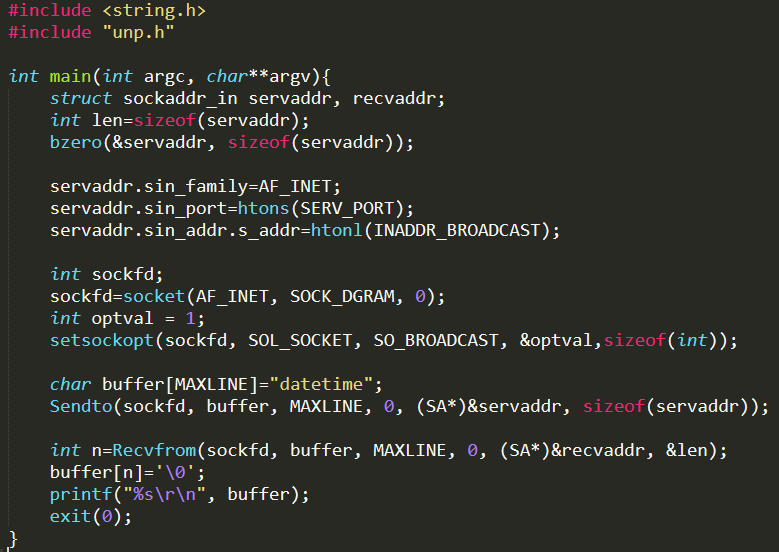
\includegraphics[width=\textwidth]{pic/broadcastc.PNG}
\caption{UDP广播客户端代码}
\end{figure}

datetime广播服务器:

1. 创建sockaddr\_in结构体,设置协议族、端口,sin\_addr.s\_addr设置为INADDR\_ANY。

2. 创建一个UDP套接口,将该套接口与上一步中的sockaddr\_in进行绑定。

3. 等待客户端请求。

4. 接收到客户端请求后,判断内容是否为"datetime",若不是则不发出响应,若是则进行响应。

5. 通过ctime()获取当前时间。

6. 将字符串形式的时间返回给客户端,之后重新进入等待客户端请求状态


\begin{figure}[H]
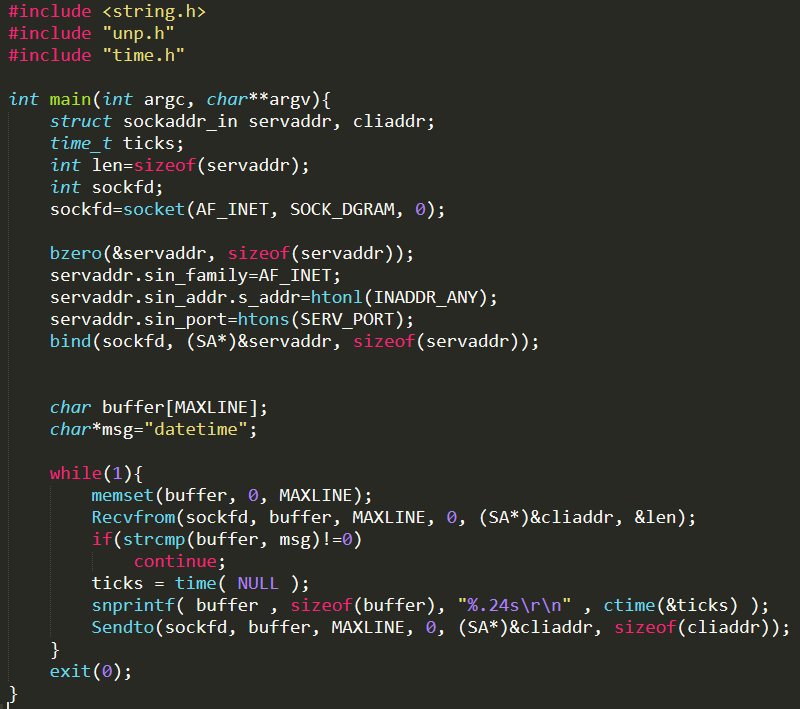
\includegraphics[width=\textwidth]{pic/broadcasts.PNG}
\caption{UDP广播服务端代码}
\end{figure}

\begin{figure}[H]
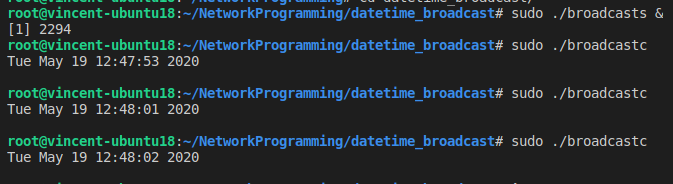
\includegraphics[width=\textwidth]{pic/broadcast_result.PNG}
\caption{广播程序运行结果}
\end{figure}

\section*{四、实验总结}

UDP广播程序与非广播程序差别不大,无需指定目标地址,只需要对发送广播的套接口设置广播属性即可。



\end{document}